% Options for packages loaded elsewhere
\PassOptionsToPackage{unicode}{hyperref}
\PassOptionsToPackage{hyphens}{url}
\PassOptionsToPackage{dvipsnames,svgnames*,x11names*}{xcolor}
%
\documentclass[
]{article}
\usepackage{lmodern}
\usepackage{amssymb,amsmath}
\usepackage{ifxetex,ifluatex}
\ifnum 0\ifxetex 1\fi\ifluatex 1\fi=0 % if pdftex
  \usepackage[T1]{fontenc}
  \usepackage[utf8]{inputenc}
  \usepackage{textcomp} % provide euro and other symbols
\else % if luatex or xetex
  \usepackage{unicode-math}
  \defaultfontfeatures{Scale=MatchLowercase}
  \defaultfontfeatures[\rmfamily]{Ligatures=TeX,Scale=1}
\fi
% Use upquote if available, for straight quotes in verbatim environments
\IfFileExists{upquote.sty}{\usepackage{upquote}}{}
\IfFileExists{microtype.sty}{% use microtype if available
  \usepackage[]{microtype}
  \UseMicrotypeSet[protrusion]{basicmath} % disable protrusion for tt fonts
}{}
\makeatletter
\@ifundefined{KOMAClassName}{% if non-KOMA class
  \IfFileExists{parskip.sty}{%
    \usepackage{parskip}
  }{% else
    \setlength{\parindent}{0pt}
    \setlength{\parskip}{6pt plus 2pt minus 1pt}}
}{% if KOMA class
  \KOMAoptions{parskip=half}}
\makeatother
\usepackage{xcolor}
\IfFileExists{xurl.sty}{\usepackage{xurl}}{} % add URL line breaks if available
\IfFileExists{bookmark.sty}{\usepackage{bookmark}}{\usepackage{hyperref}}
\hypersetup{
  pdftitle={Extra Tutorial: R Markdown},
  pdfauthor={Semuhi Sinanoglu},
  colorlinks=true,
  linkcolor=Maroon,
  filecolor=Maroon,
  citecolor=Blue,
  urlcolor=blue,
  pdfcreator={LaTeX via pandoc}}
\urlstyle{same} % disable monospaced font for URLs
\usepackage[margin=1in]{geometry}
\usepackage{color}
\usepackage{fancyvrb}
\newcommand{\VerbBar}{|}
\newcommand{\VERB}{\Verb[commandchars=\\\{\}]}
\DefineVerbatimEnvironment{Highlighting}{Verbatim}{commandchars=\\\{\}}
% Add ',fontsize=\small' for more characters per line
\usepackage{framed}
\definecolor{shadecolor}{RGB}{248,248,248}
\newenvironment{Shaded}{\begin{snugshade}}{\end{snugshade}}
\newcommand{\AlertTok}[1]{\textcolor[rgb]{0.94,0.16,0.16}{#1}}
\newcommand{\AnnotationTok}[1]{\textcolor[rgb]{0.56,0.35,0.01}{\textbf{\textit{#1}}}}
\newcommand{\AttributeTok}[1]{\textcolor[rgb]{0.77,0.63,0.00}{#1}}
\newcommand{\BaseNTok}[1]{\textcolor[rgb]{0.00,0.00,0.81}{#1}}
\newcommand{\BuiltInTok}[1]{#1}
\newcommand{\CharTok}[1]{\textcolor[rgb]{0.31,0.60,0.02}{#1}}
\newcommand{\CommentTok}[1]{\textcolor[rgb]{0.56,0.35,0.01}{\textit{#1}}}
\newcommand{\CommentVarTok}[1]{\textcolor[rgb]{0.56,0.35,0.01}{\textbf{\textit{#1}}}}
\newcommand{\ConstantTok}[1]{\textcolor[rgb]{0.00,0.00,0.00}{#1}}
\newcommand{\ControlFlowTok}[1]{\textcolor[rgb]{0.13,0.29,0.53}{\textbf{#1}}}
\newcommand{\DataTypeTok}[1]{\textcolor[rgb]{0.13,0.29,0.53}{#1}}
\newcommand{\DecValTok}[1]{\textcolor[rgb]{0.00,0.00,0.81}{#1}}
\newcommand{\DocumentationTok}[1]{\textcolor[rgb]{0.56,0.35,0.01}{\textbf{\textit{#1}}}}
\newcommand{\ErrorTok}[1]{\textcolor[rgb]{0.64,0.00,0.00}{\textbf{#1}}}
\newcommand{\ExtensionTok}[1]{#1}
\newcommand{\FloatTok}[1]{\textcolor[rgb]{0.00,0.00,0.81}{#1}}
\newcommand{\FunctionTok}[1]{\textcolor[rgb]{0.00,0.00,0.00}{#1}}
\newcommand{\ImportTok}[1]{#1}
\newcommand{\InformationTok}[1]{\textcolor[rgb]{0.56,0.35,0.01}{\textbf{\textit{#1}}}}
\newcommand{\KeywordTok}[1]{\textcolor[rgb]{0.13,0.29,0.53}{\textbf{#1}}}
\newcommand{\NormalTok}[1]{#1}
\newcommand{\OperatorTok}[1]{\textcolor[rgb]{0.81,0.36,0.00}{\textbf{#1}}}
\newcommand{\OtherTok}[1]{\textcolor[rgb]{0.56,0.35,0.01}{#1}}
\newcommand{\PreprocessorTok}[1]{\textcolor[rgb]{0.56,0.35,0.01}{\textit{#1}}}
\newcommand{\RegionMarkerTok}[1]{#1}
\newcommand{\SpecialCharTok}[1]{\textcolor[rgb]{0.00,0.00,0.00}{#1}}
\newcommand{\SpecialStringTok}[1]{\textcolor[rgb]{0.31,0.60,0.02}{#1}}
\newcommand{\StringTok}[1]{\textcolor[rgb]{0.31,0.60,0.02}{#1}}
\newcommand{\VariableTok}[1]{\textcolor[rgb]{0.00,0.00,0.00}{#1}}
\newcommand{\VerbatimStringTok}[1]{\textcolor[rgb]{0.31,0.60,0.02}{#1}}
\newcommand{\WarningTok}[1]{\textcolor[rgb]{0.56,0.35,0.01}{\textbf{\textit{#1}}}}
\usepackage{longtable,booktabs}
% Correct order of tables after \paragraph or \subparagraph
\usepackage{etoolbox}
\makeatletter
\patchcmd\longtable{\par}{\if@noskipsec\mbox{}\fi\par}{}{}
\makeatother
% Allow footnotes in longtable head/foot
\IfFileExists{footnotehyper.sty}{\usepackage{footnotehyper}}{\usepackage{footnote}}
\makesavenoteenv{longtable}
\usepackage{graphicx,grffile}
\makeatletter
\def\maxwidth{\ifdim\Gin@nat@width>\linewidth\linewidth\else\Gin@nat@width\fi}
\def\maxheight{\ifdim\Gin@nat@height>\textheight\textheight\else\Gin@nat@height\fi}
\makeatother
% Scale images if necessary, so that they will not overflow the page
% margins by default, and it is still possible to overwrite the defaults
% using explicit options in \includegraphics[width, height, ...]{}
\setkeys{Gin}{width=\maxwidth,height=\maxheight,keepaspectratio}
% Set default figure placement to htbp
\makeatletter
\def\fps@figure{htbp}
\makeatother
\setlength{\emergencystretch}{3em} % prevent overfull lines
\providecommand{\tightlist}{%
  \setlength{\itemsep}{0pt}\setlength{\parskip}{0pt}}
\setcounter{secnumdepth}{-\maxdimen} % remove section numbering
\usepackage{placeins}
\usepackage{ragged2e}
\usepackage{booktabs}
\usepackage{longtable}
\usepackage{array}
\usepackage{multirow}
\usepackage{wrapfig}
\usepackage{float}
\usepackage{colortbl}
\usepackage{pdflscape}
\usepackage{tabu}
\usepackage{threeparttable}
\usepackage{threeparttablex}
\usepackage[normalem]{ulem}
\usepackage{makecell}

\title{Extra Tutorial: R Markdown}
\author{Semuhi Sinanoglu}
\date{September 2020}

\begin{document}
\maketitle

\hypertarget{q1}{%
\section{Q1}\label{q1}}

\hypertarget{answer-to-1.1-subheading}{%
\subsection{Answer to 1.1 (subheading)}\label{answer-to-1.1-subheading}}

\begin{Shaded}
\begin{Highlighting}[]
\CommentTok{#eval: to run the code or not}
\CommentTok{#you can suppress the results of this chunk or show it as it is, or you write 'hide'}
\CommentTok{#you can hide the code in your final output through echo}
\CommentTok{#suppress messages automatically displayed when you run a code like acknowledgements}

\NormalTok{schools <-}\StringTok{ }\KeywordTok{expand.grid}\NormalTok{(}\DataTypeTok{status=}\KeywordTok{c}\NormalTok{(}\StringTok{"Public"}\NormalTok{, }\StringTok{"Private"}\NormalTok{), }
                       \DataTypeTok{funding=}\KeywordTok{seq}\NormalTok{(}\DecValTok{1500}\NormalTok{, }\DecValTok{2000}\NormalTok{, }\DataTypeTok{by=}\DecValTok{100}\NormalTok{), }
                       \DataTypeTok{teacher=}\KeywordTok{c}\NormalTok{(}\KeywordTok{seq}\NormalTok{(}\DecValTok{5}\NormalTok{,}\DecValTok{15}\NormalTok{,}\DataTypeTok{by=}\DecValTok{5}\NormalTok{),}\OtherTok{NA}\NormalTok{)) }

\KeywordTok{mean}\NormalTok{(schools}\OperatorTok{$}\NormalTok{teacher, }\DataTypeTok{na.rm =} \OtherTok{TRUE}\NormalTok{)}
\end{Highlighting}
\end{Shaded}

\hypertarget{q2}{%
\section{Q2}\label{q2}}

You can drop your comments here. For a new line:\\

You can write mathematical equations like this:
\(20 \geq \alpha \geq 76\).\\
You can make \textbf{things bold} or \emph{italic}.

For hyperlinks: \href{https://www.r-project.org/}{R project}

If you want to leave some larger gap:

\(~\)

You can itemize:

\begin{itemize}
\tightlist
\item
  Like this\ldots{}
\item
  And this\ldots{}
\item
  and goes on\ldots{}
\end{itemize}

Another kind of listing:

\begin{enumerate}
\def\labelenumi{\arabic{enumi}.}
\tightlist
\item
  Coding is fun.
\item
  Yes, I mean it.
\item
  Hang in there!
\end{enumerate}

\hypertarget{q3}{%
\section{Q3}\label{q3}}

\hypertarget{how-to-create-a-table}{%
\subsection{How to create a table}\label{how-to-create-a-table}}

There are different ways in which you can create tables. If you want to
create a table of an existing dataset, use the kable function.

I will not show you all the details, but you can put multiple tables
side by side. Literally change anything with the outlook of your table
with kable and kableExtra packages.

\begin{table}[!h]

\caption{\label{tab:table}Minimum wage dataset}
\centering
\fontsize{10}{12}\selectfont
\begin{tabular}[t]{lccccccc}
\toprule
chain & location & wageBefore & wageAfter & fullBefore & fullAfter & partBefore & partAfter\\
\midrule
\cellcolor{gray!6}{wendys} & \cellcolor{gray!6}{PA} & \cellcolor{gray!6}{5.00} & \cellcolor{gray!6}{5.25} & \cellcolor{gray!6}{20.0} & \cellcolor{gray!6}{0} & \cellcolor{gray!6}{20} & \cellcolor{gray!6}{36}\\
wendys & PA & 5.50 & 4.75 & 6.0 & 28 & 26 & 3\\
\cellcolor{gray!6}{burgerking} & \cellcolor{gray!6}{PA} & \cellcolor{gray!6}{5.00} & \cellcolor{gray!6}{4.75} & \cellcolor{gray!6}{50.0} & \cellcolor{gray!6}{15} & \cellcolor{gray!6}{35} & \cellcolor{gray!6}{18}\\
burgerking & PA & 5.00 & 5.00 & 10.0 & 26 & 17 & 9\\
\cellcolor{gray!6}{kfc} & \cellcolor{gray!6}{PA} & \cellcolor{gray!6}{5.25} & \cellcolor{gray!6}{5.00} & \cellcolor{gray!6}{2.0} & \cellcolor{gray!6}{3} & \cellcolor{gray!6}{8} & \cellcolor{gray!6}{12}\\
\addlinespace
kfc & PA & 5.00 & 5.00 & 2.0 & 2 & 10 & 9\\
\cellcolor{gray!6}{roys} & \cellcolor{gray!6}{PA} & \cellcolor{gray!6}{5.00} & \cellcolor{gray!6}{4.75} & \cellcolor{gray!6}{2.5} & \cellcolor{gray!6}{1} & \cellcolor{gray!6}{20} & \cellcolor{gray!6}{25}\\
burgerking & PA & 5.00 & 5.00 & 40.0 & 9 & 30 & 32\\
\cellcolor{gray!6}{burgerking} & \cellcolor{gray!6}{PA} & \cellcolor{gray!6}{5.00} & \cellcolor{gray!6}{4.50} & \cellcolor{gray!6}{8.0} & \cellcolor{gray!6}{7} & \cellcolor{gray!6}{27} & \cellcolor{gray!6}{39}\\
burgerking & PA & 5.50 & 4.75 & 10.5 & 18 & 30 & 10\\
\bottomrule
\end{tabular}
\end{table}

\newpage

\begin{longtable}[]{@{}ll@{}}
\toprule
Name & Description\tabularnewline
\midrule
\endhead
\texttt{election\_id} & Unique identifier for each
election\tabularnewline
\texttt{country} &\tabularnewline
\texttt{year} &\tabularnewline
\texttt{party\_name} & Name of the political party translated to
English\tabularnewline
\texttt{vote\_share} & Votes for the party as a percentage of total
cast\tabularnewline
\texttt{seats} & The number of seats the party won\tabularnewline
\texttt{seats\_total} & Total seats obtained in an election (for all
parties)\tabularnewline
\texttt{left\_right} & Average left-right ideology from a variety of
sources (higher = more right)\tabularnewline
\texttt{state\_market} & Average economic left-right score from two
sources (higher = more right)\tabularnewline
\texttt{liberty\_authority} & Average social left-right score from two
sources (higher = more right)\tabularnewline
\texttt{party\_family} & Party family\tabularnewline
\texttt{halfdecade} & Five-year intervals to make aggregation
easier\tabularnewline
\bottomrule
\end{longtable}

\begin{longtable}[]{@{}ll@{}}
\toprule
\textbf{Date} & \textbf{Cases}\tabularnewline
\midrule
\endhead
30/8/2020 & 371\tabularnewline
29/8/2020 & 350\tabularnewline
28/8/2020 & 300\tabularnewline
27/8/2020 & 267\tabularnewline
26/8/2020 & 226\tabularnewline
25/8/2020 & 192\tabularnewline
24/8/2020 & 174\tabularnewline
\bottomrule
\end{longtable}

\centering

\textbf{Table: COVID cases in Toronto} \justify

You can set figure width and height: \FloatBarrier

\begin{Shaded}
\begin{Highlighting}[]
\KeywordTok{plot}\NormalTok{(}\KeywordTok{density}\NormalTok{(}\KeywordTok{rnorm}\NormalTok{(}\DecValTok{1000}\NormalTok{)), }\DataTypeTok{main =} \StringTok{"1000 Draws from a Standard Normal"}\NormalTok{)}
\end{Highlighting}
\end{Shaded}

\begin{center}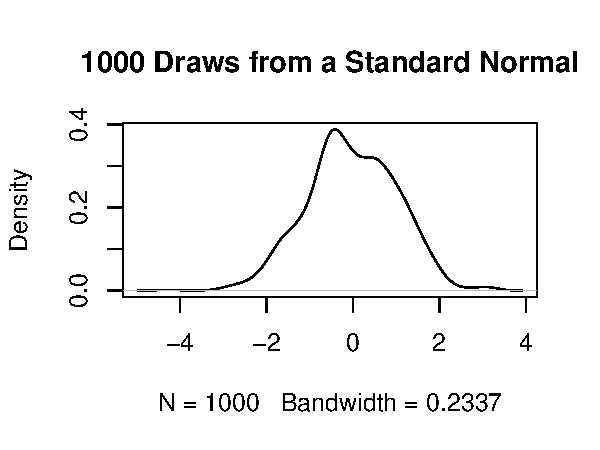
\includegraphics{extra-tutorial-markdown_files/figure-latex/unnamed-chunk-1-1} \end{center}

\end{document}
